% The end-to-end retrieval-augmented generation (RAG) architecture of Lewis et al. (2020).
\begin{figure*}[t]
\centering
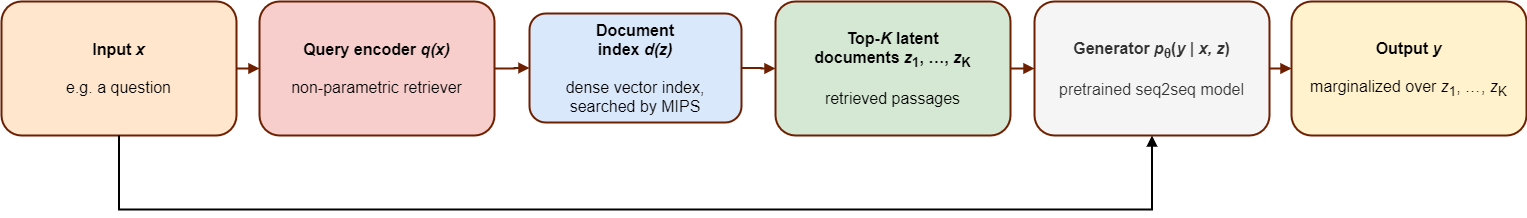
\includegraphics[width=\textwidth]{images/rag_original_architecture.png}
\caption{The end-to-end retrieval-augmented generation (RAG) architecture of
\citet{lewis2020}, redrawn here for discussion. A non-parametric retriever ($q(x)$ over a dense
document index $d(z)$, searched with Maximum Inner Product Search) returns the top-$K$ passages
for an input $x$; a parametric seq2seq generator then conditions on both $x$ and each retrieved
passage and the final output $y$ is marginalized over the retrieved set. This general-domain
architecture, not originally designed for law, is the direct ancestor of every legal RAG pipeline
discussed in the remainder of this survey.}
\label{fig:lewis-rag}
\end{figure*}
